\chapter{Coding}

\section{Assembly}

In order to get the CPU to do some of what we've discussed above, it needs to have code loaded onto it to run. We write code in a language called assembly. Assembly is a human-readable language. A program is made up of a sequence of instruction; each instruction gets executed by the CPU. It's quite easy to see what each instruction does by reading the program.  The complete instruction set is located in the Programming Manual. You must be familiar with this document! Examples of instruction which carry out the tasks listed above are:
\begin{enumerate}
  \item \texttt{ADDS R6, R0, R1}
  \item \texttt{MOV R0, R3}
  \item \texttt{EORS R3, R3, R4}
  \item \texttt{MOVS R5, \#42}
\end{enumerate}
The CPU does not have the ability to understand our nice English words like \textit{ADD} or \textit{MOV}. The CPU only has the ability to understand binary data. Assembly code must be compiled to machine code. A machine code instruction is a binary string, 16 bits long consisting of the operation code (opcode) and the data which it must operate on (operand).
For example, assume that we wanted to ascertain the machine code representation of the instruction \texttt{ADDS R6, R0, R1}. An extact from the ARMv6-M Architecture Reference Manual is shown in \autoref{fig:adds_encoding} where Rd is the destination register and Rm and Rn are the source registers of the add. It can easily be seen that the instruction would compile to\texttt{ 0001100 001 000 110 = 0x1846}.
\begin{figure}
\centering
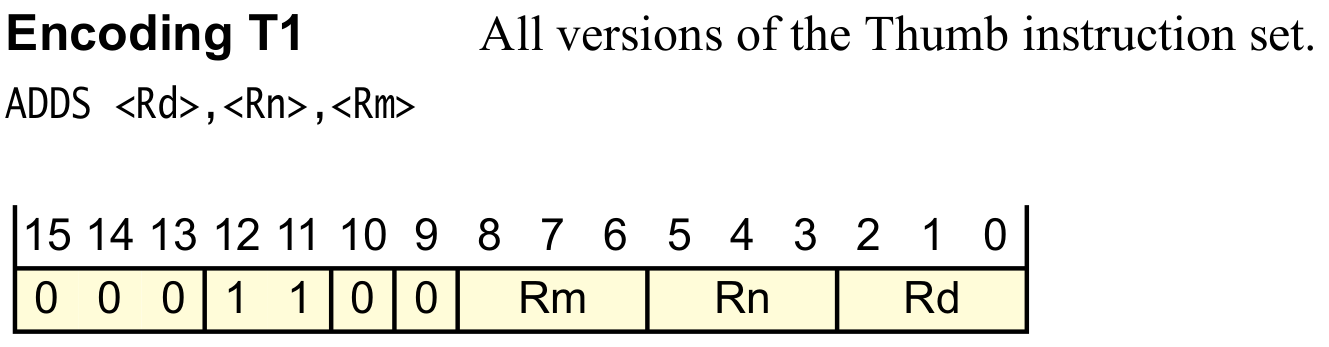
\includegraphics[width=0.7\textwidth]{./week1/adds_encoding}
\caption{An encoding of the ADDS instruction}
\label{fig:adds_encoding}
\end{figure}
The opcodes for each instruction are detailed in the ARMv6-M Architecture Reference Manual.
All of the instructions in the program are 16 bits long and are stored sequentially after one another in flash memory. 


\subsection{Instruction Sets}
An instruction set is the collection of all of the instructions which a processor can execute. 
The ARM Cortex-M0 uses the ARMv6-M architecture and this architecture supports the Thumb instruction set (as opposed to Thumb-2 or ARM). 
Thumb contains about \emph{XXX} instructions, each of which is 16 bits long. \\

Higher end ARM processors such as the Cortex-M3 or Cortex-M4 support the ARMv7-M architecture which allows multiple instruction sets to be supported by the processor. 
The ability to support multiple instruction sets requires \emph{interworking}. Interworking is the ability to specify to the CPU which instruction set to use. 
While our ARM Cortex-M0 only supports the Thumb instruction set, there is no need for interworking, yet the cabability has still been incorperated into the architecture to allow for compatability to other processors. 
This means that although our processor only supports one instruction set (Thumb), we have to explicity tell it that we are using that instruction set. 


\section{Linking}
Once our assembly code has been written and compiled to machine code, the computer which loads the code onto the micro has to be told what addresses to place the code at. The code should be placed starting at the beginning of flash.

\subsection{Executing Code}
Once the code has been loaded onto the microcontroller, it will execute one instruction after the next. 
CPU register R15 is reserved for keeping track of where the micro is in execution. It is known as the Program Counter (PC).
The PC always points to the instruction which is ABOUT to be executed. Hence, when your micro boots up, before it has executed anything, the PC will point to the first instruction to be executed.
By ``point to'' we mean that it holds the address of the instruction. 

As each instruction in the ARM Cortex-M0 instruction set it 16 bits (aka: half a word) long, ARM have implemented a rule that all instructions must be half word alligned. In other words, the address of the instruction must be divisible by 2 bytes. Legal addresses for instructions are hence, 0x02, 0x04, 0x06, 0x08 ... etc. 
This means that the least significant bit (bit 0) of the PC register is unused in specifcying the address of an instruction. 
Hence, it has been assigned another use. Specifically, to indicate the type of instruction which is being executed. 


